\chapter{Background and literature search}

There are lots of different algorithms and approaches existing in the field of object detection and tracking. Some of those algorithms were investigated in this project in order to identify a set of suitable algorithms that were both accurate and efficient enough to analysis video stream from camera by an embedded platform in real time.

Object tracking typically consists of 2 steps. Initially, locations and shapes of each moving object appeared in each frame need to be identified. Subsequently, by analysing and recording the movements of each object in sequential frames, the objects in a video stream can be tracked.

\section{OpenCV computer vision library}

% {\color{red}Information...}

OpenCV computer vision library \cite{opencv} is a very powerful open-source computer vision library. It contains lots of useful computer vision algorithms, designed for computational efficiency and real-time applications, mostly platform independent and can take the advantage of multi-core and GPU parallel processing on heterogeneous platforms.

\section{Model based object detection algorithms}

\iffalse
Being able to detect objects in a video frame is the first, also the most important and challenging step to do object tracking. This is generally accomplished by separation of foreground objects and background image.
\fi

Object detection is generally accomplished by separation of foreground and background masks, called background subtraction or foreground segmentation.

\subsection{Colour based}
\label{bgs:colour}

Colour can sometimes provide enough information about a specific object, for example a coloured ball. For filtering a specific colour out from a video frame, hue-saturation-value (HSV) colour space \cite[p.~301]{colourspace} representation is usually used, which can make colour filtering a lot easier based on hue, saturation and brightness information of the specific colour. In this way, a foreground mask can be generated easily by filtering target colour. For example, \fref{Figure:MOTBOC} shows a simple colour filtering object detection implementation \cite{MOTBOC.git} that is able to detect objects with specific colours.

\begin{figure}[H]
  \centering
  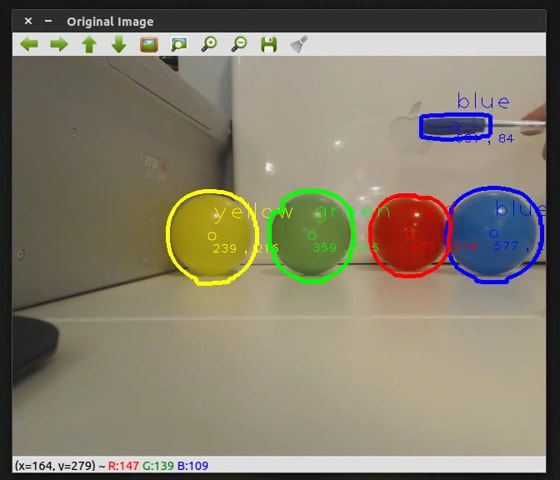
\includegraphics[width=0.5\columnwidth]{MOTBOC}
  \caption{Multi object tracking based on colour filtering (sourced from \cite{MOTBOC.git}).}
  \label{Figure:MOTBOC}
\end{figure}

This implementation does not require a lot of graphic processing, thus can be made very quick and efficient, suitable for robots that are tracking something like a coloured ball or piece of paper, also could be useful for line racing car projects.

There are also researches using a more complex particle filtering algorithm based on colour distributions over a region in the frame \cite{nummiaro2003color}, results shown by \fref{Figure:nummiaro2003color}. The cameras need to be calibrated and compensated first, then a colour distribution model of the target object need to be built, then the elliptical region of the tracked object get determined by apply colour-based particle filters \cite{nummiaro2003adaptive}. The algorithm from the research are purposed to be used in multi-camera environments to select the best view of the target, therefore several views from different camera are shown by the images at the bottom, along with the coefficients implies similarity with the target model shown at the top left, and the selected best view at the top right.
% {\color{red}Details on algorithm implementation required.}

\begin{figure}[H]
  \centering
  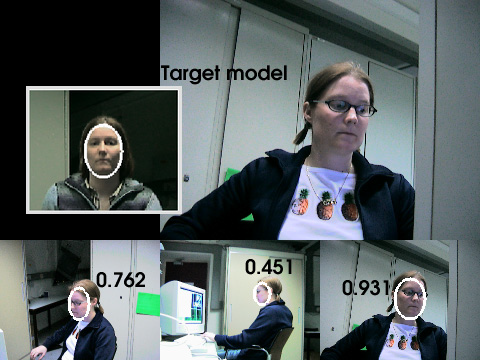
\includegraphics[width=0.5\columnwidth]{nummiaro2003color}
  \caption{Object tracking based on colour distribution particle filtering in multi-camera environments (sourced from \cite{nummiaro2003color}).}
  \label{Figure:nummiaro2003color}
\end{figure}

However, if there were other targets with similar colour distribution, the algorithm may failed to distinguish them, as shown by the second image in \fref{Figure:nummiaro2003color_fail}, the face of the man got tracked instead of the target woman's face. It also requires a specific model associated with each of the objects to be tracked.

\begin{figure}[H]
  \centering
  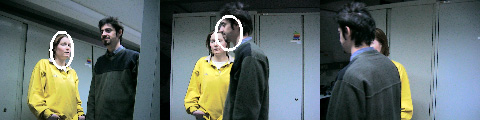
\includegraphics[width=0.9\columnwidth]{nummiaro2003color_fail}
  \caption{Problems on colour based object tracking, when several good candidates exists at the same time (sourced from \cite{nummiaro2003color}).}
  \label{Figure:nummiaro2003color_fail}
\end{figure}

\subsection{Shape matching}

Another important information about an object might be its distinctive shape. By extracting object edges in the scene than apply appropriate shape matching algorithms, an object can be detected based on its shape.

This research \cite{borovicka2003circle} shows the ability to detect circles in a image by applying edge filtering followed by Hough transforms, as shown by \fref{Figure:circles}. \fref{Figure:circle:original} shows the original grey scaled image, then after blurred and Sobel filtered (\fref{Figure:circle:sobel}), clear edges been extracted (\fref{Figure:circle:edge}). Finally, Hough transform been applied, the results merged with the original image are shown by \fref{Figure:circle:circles}.

\begin{figure}[H]
  \centering
  \subfigure [] {
    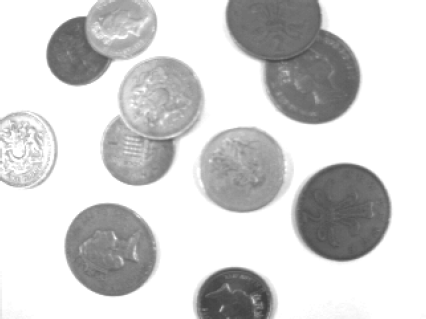
\includegraphics[width=0.22\columnwidth]{circle_original}
    \label{Figure:circle:original}
  }
  \subfigure [] {
    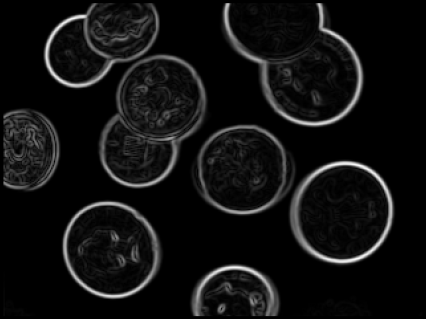
\includegraphics[width=0.22\columnwidth]{circle_sobel}
    \label{Figure:circle:sobel}
  }
  \subfigure [] {
    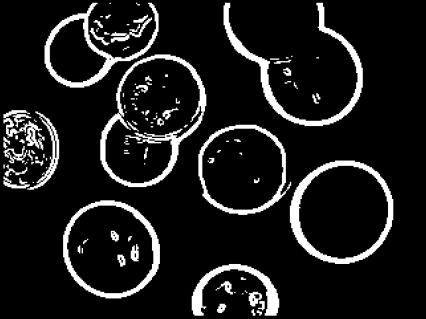
\includegraphics[width=0.22\columnwidth]{circle_edge}
    \label{Figure:circle:edge}
  }
  \subfigure [] {
    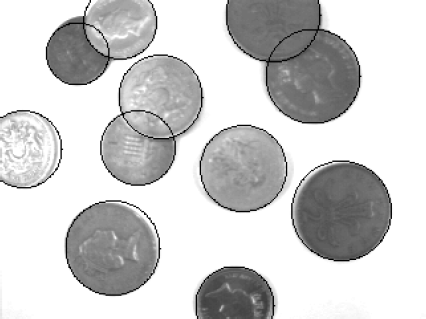
\includegraphics[width=0.22\columnwidth]{circle_circles}
    \label{Figure:circle:circles}
  }
  \caption{Circle detection by Hough transform (sourced from \cite{borovicka2003circle}). \subref{Figure:circle:original} shows the original image, \subref{Figure:circle:sobel} Sobel filters applied, \subref{Figure:circle:edge} threshold edge map, \subref{Figure:circle:circles} detected circles}
  \label{Figure:bg_circles}
\end{figure}

This implementation might be suitable for ball tracking purpose. By combining with the colour filtering as described in Section \ref{bgs:colour}, a single coloured ball could be efficiently tracked.

\subsection{Feature detection (Cascaded classifier)}
\label{sec:bg:cc}

% {\color{red}Use this: \cite{viola2001rapid}}

Cascade classifier \cite{cascade} \cite{viola2001rapid} is a widely used object detection technique based on machine learning. By concatenating a large number of simple feature detectors (i.e. classifiers) each detecting different simple features based on intensity at different positions as shown by \fref{bg:cc}, complex objects such as human faces can be recognised as shown in \fref{bg:cc:faces}. Furthermore its accuracy can be improved by training the classifier both positively and negatively.

\begin{figure}[H]
  \centering
  \subfigure [] {
    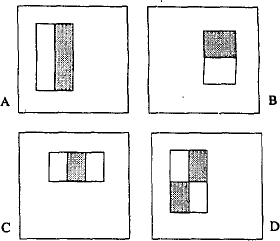
\includegraphics[width=0.3\columnwidth]{cc_features}
    \label{bg:cc:features}
  }
  \subfigure [] {
    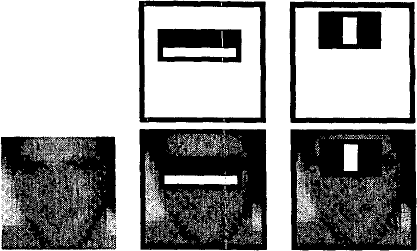
\includegraphics[width=0.3\columnwidth]{cc_face}
    \label{bg:cc:face}
  }
  \caption{Cascade classifier (sourced from \cite{borovicka2003circle}). \subref{bg:cc:features} shows some example simple feature detector configurations, \subref{bg:cc:face} shows some feature detector used on face recognition.}
  \label{bg:cc}
\end{figure}

\begin{figure}[H]
  \centering
  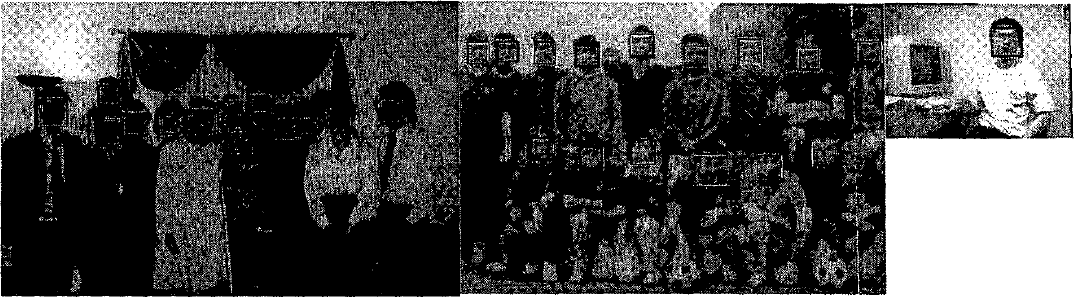
\includegraphics[width=0.9\columnwidth]{cc_faces}
  \caption{Cascade classifier recognising human faces (sourced from \cite{borovicka2003circle}).}
  \label{cc:faces}
\end{figure}

This algorithm is mostly used for object classification, for example recognising human faces, bodies and different classes of vehicles in images. Like other model based algorithms, multiple classifier definitions are required for detecting different kinds of objects, or even different perspectives of the same object.

% {\color{red}Replace with results from research paper}

\section{Motion based object detection algorithms}

\subsection{Background subtraction}
\label{motion_bs}

By studying frames from a video stream then build up a background model image, it is also possible to detect moving objects in following frames efficiently.

% {\color{red}Add some graph from research paper?}

% {\color{red}Should be in design section?

% This type of algorithms suit well for static camera movement tracking, and were not limited by objects' geometry shapes, therefore was used in this project.}

% {\color{cyan}Background subtraction algorithms:

There are several background subtraction algorithms available, the BGSLibrary \cite{bgslibrary} is specifically developed for analysis those algorithms, it offers 37 different background subtraction algorithms implemented using OpenCV, published under GNU GPL v3 license. With the same programming interface for all available algorithms, it allows easy swapping between algorithms.

There is an article \cite{bgs:article} reviewed the algorithms available in the BGSLibrary, ranked 5 algorithms as the best in overall performance score as shown in \tref{Table:bgs}. \fref{bgsreview} shows foreground masks obtained from the top 5 algorithms on sequences from real world videos at the same frame. TP pixels means foreground pixels classified as foreground, TN pixels background pixels classified as background which are correct results, whereas FP pixels means background pixels classified as foreground, and FN pixels means foreground pixels classified as background which are incorrect results. The actual foreground masks generated by the algorithms are TP and FN pixels.

\begin{table}[H]
  \centering
  \begin{tabular}{cc}
  \toprule
  \textbf{Method ID} & \textbf{Method name}\\
  \midrule
  PBAS & Pixel-Based Adaptive Segmenter \\
  MultiLayerBGS & Multi-Layer BGS \\
  MixtureOfGaussianV1BGS & Gaussian Mixture Model \\
  LBAdaptiveSOM & Adaptive SOM \\
  DPWrenGABGS & Gaussian Average \\
  \bottomrule
  \end{tabular}
  \caption{Background substraction algorithms investigated (adapted from \cite{bgslibrary})}
  \label{Table:bgs}
\end{table}

\begin{figure}[tbh]
  \centering
  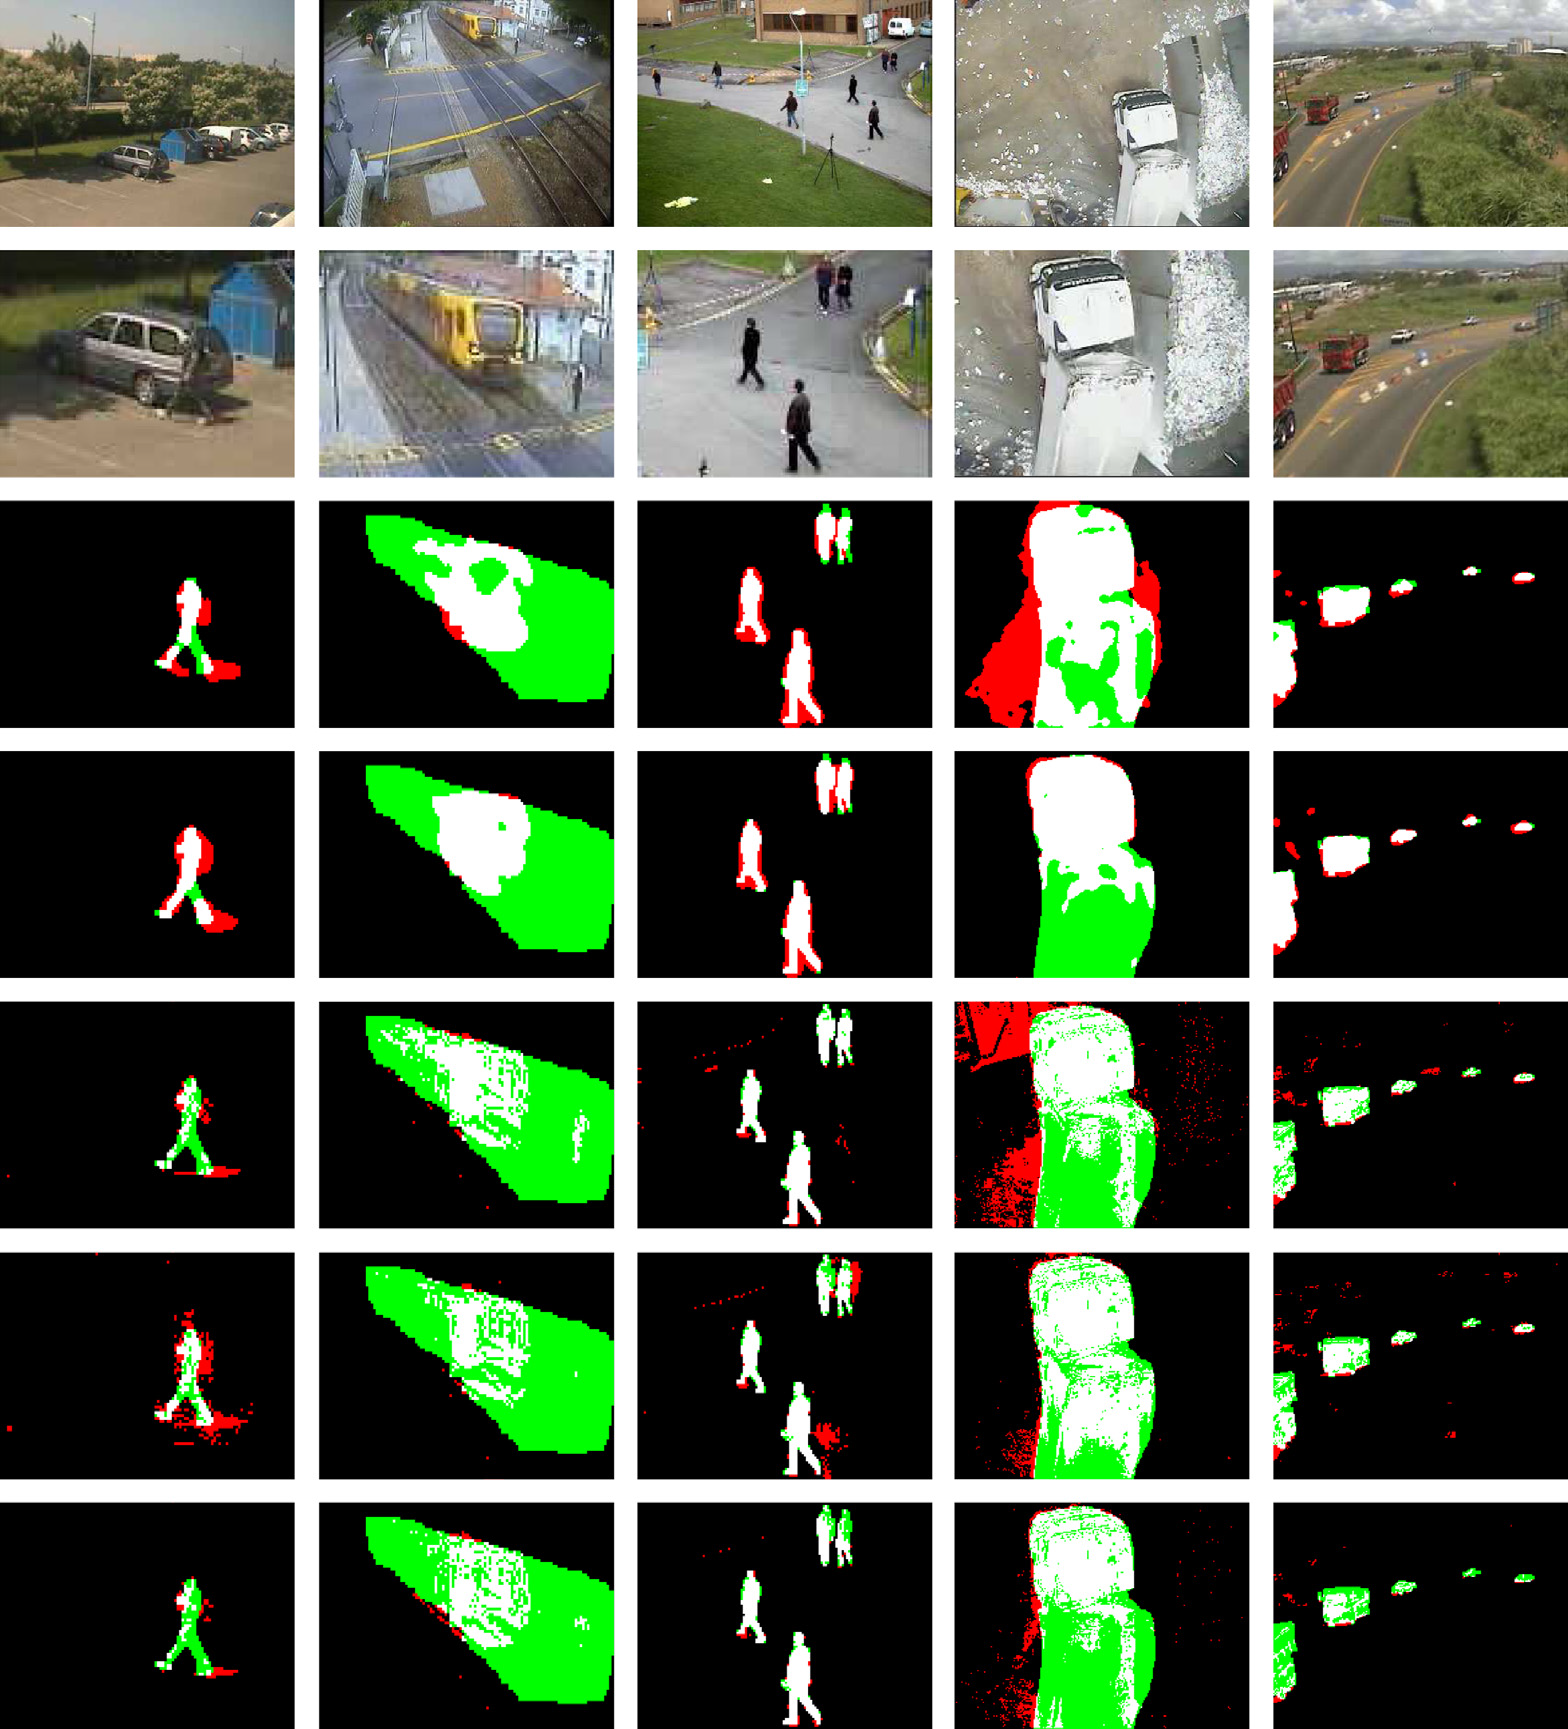
\includegraphics[width=0.9\columnwidth]{bgsreview}
  \caption{Foreground masks obtained from 5 different background subtraction algorithms from real world videos (sourced from \cite{bgs:article}). Images from the first to last row are the input frame, region of interest zoomed in, PBAS, MultiLayerBGS, LBAdaptiveSOM, DPWrenGABGS and MixtureOfGaussianV1BGS algorithms. For the colours, TP pixels are in white, TN pixels are in black, FP pixels are in red, and FN pixels are in green.}
  \label{bgsreview}
\end{figure}

Unfortunately, the PBAS algorithm is no longer available in the BGSLibrary, it is based on the patented ViBE algorithm \cite{barnich2011vibe} therefore was removed because of patent issues. The ViBE algorithm is a powerful background subtraction algorithm with very fast processing speed, high precision and moderate memory usage, the initial implementation is still available, and was existed in early versions of OpenCV implemented with CUDA codes runs on GPU.
%}

\iffalse
\subsection{Optical flow}

Optical flow is another widely used object tracking algorithm, it can be used for detect moving objects as well.

There are 2 types of optical flow algorithms. One is sparse feature set (Lucas-Kanade method \cite{bouguet2001pyramidal}), it evaluates pixel movements around selected feature points, therefore calculates movements of feature points. Another type is dense optical flow (Gunner Farneback's algorithm \cite{farneback2003two}), it evaluates pixel movements for all pixels in the frame.

{\color{red}More descriptions and images?}

By rendering pixel movements in 3 axes computed from dense optical flow as 3 components (RGB) colours, then find out regions with the same colour, sizes and positions of moving objects in the scene can then be determined. However, once an object stopped moving, the optical flow algorithms cannot distinguish the object from background any longer.
\fi

\section{Object tracking algorithms}
\label{bg:tracking}

\subsection{Connected component analysis}
\label{blob}

After obtained the foreground object mask by one of the methods described above, it need to be interpreted as distinct objects, so that the geometry properties of each object can then be retrieved.

Connected component analysis, or connected component labelling, is used for detecting regions that are differ in some properties, such as colour or brightness. Such a region is also called a blob, which can be the possible presence region of an independent object if applied to the foreground masks. It is very useful to extract parameters such as shape, size and location of the object afterwards.

There are open source blob detection libraries available, such as the simple blob detector came with OpenCV \cite{opencv:blob}, and the cvBlob library \cite{cvblob}. \fref{cvblob} shows an example of tracking blobs by using the cvBlob library.

%{\color{red}Images}

\begin{figure}[H]
  \centering
  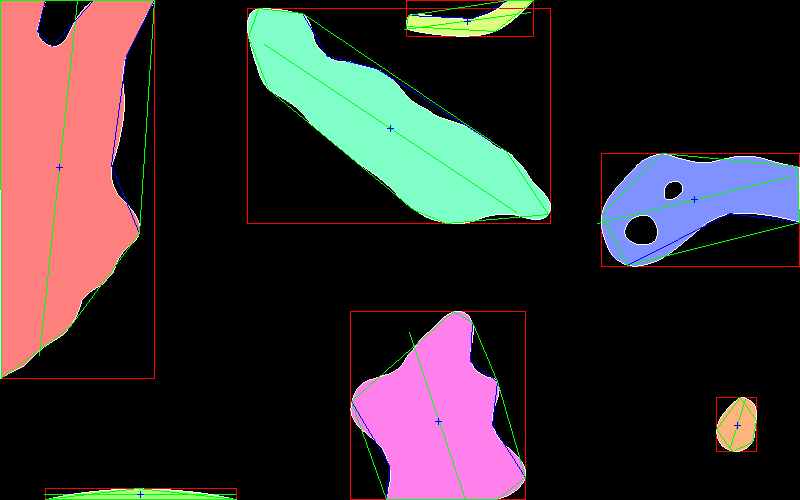
\includegraphics[width=0.7\columnwidth]{cvblob}
  \caption{Tracking blobs with the cvBlob library with bounding shapes, bounding rectangles and blob centres shown (sourced from \cite{cvblob}).}
  \label{cvblob}
\end{figure}

After determined the bounding shape, or region of interest (ROI) of an object, the object can then be tracked between adjacent frames by matching the blobs based on similarity in colour and shape or relative position. Movement parameter such as velocity and acceleration may also be obtained by physical modelling.

\subsection{Meanshift and CAMshift}

Meanshift \cite{fukunaga2013introduction} is an algorithm can be used to track the movement of a fixed size ROI window between adjacent frames. To accomplish this, histogram back projection need to be applied first to the new frames, which converts the frame to a probability image of each pixels belongs to the target model. Then the meanshift algorithm will be applied to find the peak of probability distribution of the target model. It was implemented within the OpenCV library \cite{opencv:camshift}. \fref{bg:ms:meanshift} shows an example tracking result.

% {\color{red}Images}

Continuously Adaptive Meanshift (CAMshift) \cite{bradski1998computer} is an algorithm based on the Meanshift algorithm, that can handle target object size changing and rotation by iterating over the ROI to find the most suitable configuration. This algorithm was also implemented in the OpenCV library \cite{opencv:camshift}, was used by lots of researches for tracking purpose, such as \cite{chu2007object}, \cite{xu2012moving} and \cite{nouar2006improved}. \fref{bg:ms:camshift} shows an example tracking result, compare to the Meanshift algorithm tracking (\fref{bg:ms:meanshift}), it can resize and rotate ROI automatically.

\begin{figure}[H]
  \centering
  \subfigure [] {
    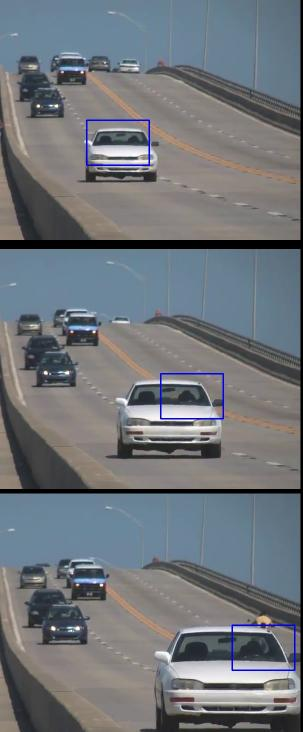
\includegraphics[width=0.3\columnwidth]{meanshift_result}
    \label{bg:ms:meanshift}
  }
  \subfigure [] {
    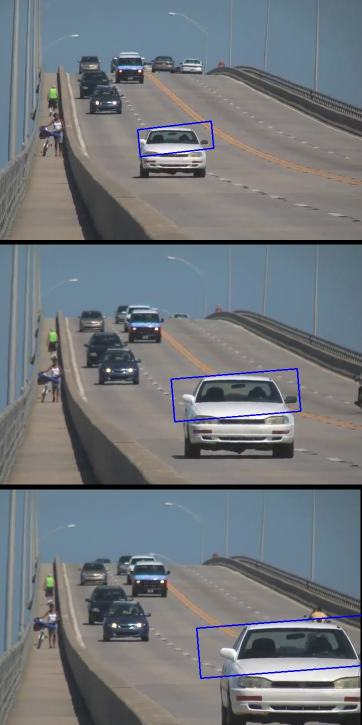
\includegraphics[width=0.35\columnwidth]{camshift_result}
    \label{bg:ms:camshift}
  }
  \caption{Meanshift and CAMshift tracking examples (sourced from \cite{opencv:camshift}). \subref{bg:ms:meanshift} shows the Meanshift tracking, \subref{bg:ms:camshift} shows the CAMshift tracking.}
  \label{bg:ms}
\end{figure}

%{\color{red}Images}

\subsection {Optical flow}

%By evaluating pixel movements of feature points inside ROI, the speeds of moving objects projected onto camera sensor can be determined.

Optical flow is another widely used object tracking algorithm that evaluates pixel moving around feature points, by assuming neighbouring pixels will have similar motion as the feature points. Although it can also be used for detecting moving objects by considering regions of points with the same motion as one moving object, however, once the object stopped moving, the optical flow algorithms cannot distinguish the object from background any longer. Therefore it is mainly used for object tracking rather than detection.

There are 2 types of optical flow algorithms. One is sparse feature set (Lucas-Kanade method \cite{bouguet2001pyramidal}), it estimates pixel movements around selected feature points. To determine feature points, OpenCV implemented a good features to track \cite{shi1994good} algorithm to find the strongest corners in an image. After that, by moving the feature points according to the movements computed, the object can be tracked across sequence of video frames, as shown by \fref{bg:of:opticalflow_lk}.

Another type is dense optical flow (Gunner Farneback's algorithm \cite{farneback2003two}), it evaluates pixel movements for all points in the frame. \fref{bg:of:opticalfb} shows the result from a dense optical flow tracking scene by rendering movements in 3 axes as red, green and blue components respectively.

\begin{figure}[H]
  \centering
  \subfigure [] {
    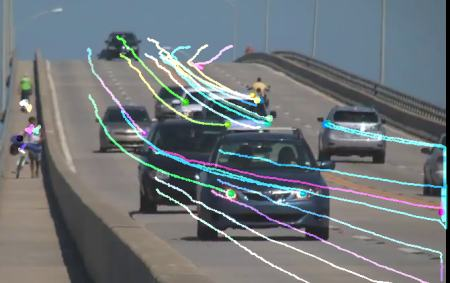
\includegraphics[width=0.3\columnwidth]{opticalflow_lk}
    \label{bg:of:opticalflow_lk}
  }
  \subfigure [] {
    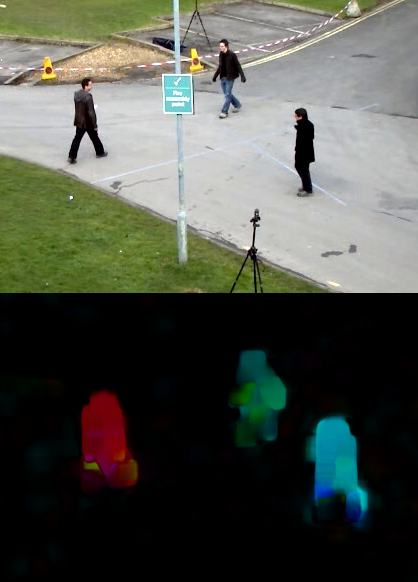
\includegraphics[width=0.3\columnwidth]{opticalfb}
    \label{bg:of:opticalfb}
  }
  \caption{Optical flow example scenes (sourced from \cite{opencv:of}). \subref{bg:of:opticalflow_lk} shows the sparse feature set (Lucas-Kanade method), \subref{bg:of:opticalfb} shows the dense optical flow (Gunner Farneback's algorithm).}
  \label{bg:of}
\end{figure}

% {\color{red}More descriptions and images?}

% {\color{red}Images}

\section{Object recognition}

Object recognition can also be developed by applying different cascade classifiers as described previously in section \ref{sec:bg:cc} to the ROI of the specific object. This process is very computation intensive and time consuming, therefore should be executed as few as possible to achieve maximum power saving, for example, only execute once when the object first enters the sense or at its maximum visible size to the camera.

\section{Automatic feedback control}

Research about energy-efficient object detection by utilising hardware-level operations exists \cite{casares2011energy}, it had achieved energy consumption reduction by $54.136\%$. However, it was done on a very different and limited platform, based on a very limited algorithm, possible to extend to algorithms with more general usage.

\section{Sample video datasets}

There are sample video datasets proposed for testing, evaluating and comparing computer vision algorithms, specifically background subtraction algorithms. The resolutions are $320 \times 240$ typically, up to about $720 \times 480$, with frame rates of $60$ frames per second (FPS) mostly.

For example, ChangeDetection.NET(CDNET) \cite{goyette2012changedetection} and Background Models Challenge \cite{vacavant2012benchmark} provides realistic camera-captured videos with lots of diverse sets of scenarios and high quality ground truth masks, while Stuttgart Artificial Background Subtraction Dataset \cite{brutzer2011evaluation} was using 3D models and ray tracing technology to generate artificial but realistic videos of typical video surveillance scenarios.
